Curve fitting is a very common theme in pattern recognition. The concept of invariant functions convey mapping functions that approximate a discriminating function when a parent function is reduced from a high dimensional space to a low dimensional space \cite{mallat2016understanding}.  In this chapter an invariance function called a scattering transform enables invariance of groups of deformations that could apply to speech signals thereby preserving higher level characterisations useful for classifying speech sounds. Works done by \citep{peddinti2014deep,zeghidour2016deep,anden2011multiscale,sainath2014deep} have shown that when the scattering spectrum are applied to speech signals and used as input to speech systems have state of the art performance.  In particular \cite{sainath2014deep} shows 4-7\% relative improvement in word error rates (WER) over Mel frequencies cepstral coefficients (MFCCs) for 50 and 430 hours of English Broadcast News speech corpus.  While experiments have been performed with hybrid HMM-DNN systems in the past, this thesis focuses on the use of scatter transforms in end-to-end RNN speech models.

This chapter iterates the use of the Fourier transform as the starting analysis function for building invariant functions and then discusses the Mel filter bank solution and then establishes why the scattering transform through the wavelet modulus operator provides better invariance features over the Mel filters.

\section{Fourier transform}
The Fourier transform often referred to as the power spectrum, allows us to discover frequencies contained within a signal.  The Fourier transform is a convolution between a signal and a complex sinusoid from $-\infty$ to $+\infty$ (Figure \ref{fig_4_1_fourier_eqn}). 

\begin{figure}
\centering
  % Requires \usepackage{graphicx}
  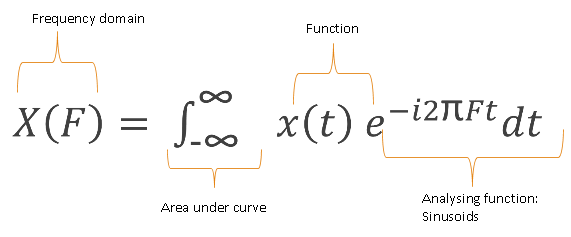
\includegraphics[width=7cm]{thesis/images/fourier.png}\\
  \caption{Fourier Equation} \label{fig_4_1_fourier_eqn}
\end{figure}
From the orthogonal property of complex exponential function, two functions are orthogonal if $\int f(x)g(x)=0$ where f(x) and g(x) are complementary functions, one being referred to as the analysis equation and the other referred to as the synthesis function.

If the discrete form of the Fourier transform analysis equation is given by
\begin{equation}
a_k=\frac{1}{T}\int_{-T/2}^{T/2}x(t)e^{\left(-j\frac{2\pi kt}{T}\right)}
\label{eqn_c4_fourier01}
\end{equation}

Then, the corresponding synthesis equation is given by
\begin{equation}
x(t)=\sum_{k=-\infty}^{\infty}a_ke^{\left(j\frac{2\pi kt}{T}\right)}
\label{eqn_c4_fourier02}
\end{equation}

Recall that $x(t)$ is the original signal while $a_k$ is the Fourier Series coefficient.  This coefficient indicates the amplitude and phase of the original signal's higher order harmonics indexed by $k$ such that higher values of $k$ correspond to higher frequency components.  In a typical spectrogram (figure \ref{fig_4_2_spectral}), it can be seen that the energy of the signal is concentrated about a central region and then harmonic spikes of energy content exponentially decrease and taper off.  Therefore in figure \ref{fig_4_2_spectral}, the energies are concentrated at frequencies of about 100, 150 and 400 hertz.
\begin{figure}
\centering
  % Requires \usepackage{graphicx}
  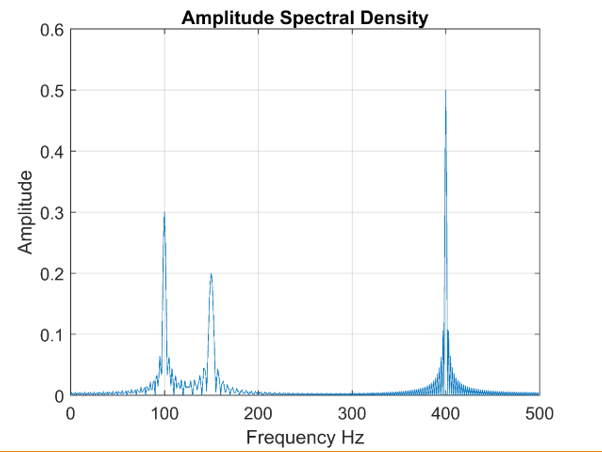
\includegraphics[width=7cm]{thesis/images/spectral.png}\\
  \caption{Sample Spectrogram} \cite{cwt_lecture}\label{fig_4_2_spectral}
\end{figure}

The Fourier transform discussed in the preceding paragraph constitutes a valuable tool for the analysis of the frequency component of a signal.  However is not able to determine when in time a frequency occurs hence is not able to analyse time related signal deformations.  The Short-time Fourier Transform (STFT) attempts to salvage this by windowing the signal in time signal and performing Fourier transforms over sliding windows sections of the original signal rather than the whole signal.  There is however, a resolution trade off that ensues from this operation such that, the higher the resolution in time accuracy, the lower the frequency accuracy and vice versa.  In the next section on the continuous wavelet transform, how the wavelet transform improves on the weaknesses of the Fourier Transform and the STFT is reviewed.

\section{Wavelet transform}
The continuous wavelet transform can be defined as a signal multiplied by scaled and shifted version of a wavelet function $\psi(t)$ referred to as the mother wavelet. The time-frequency tile-allocation of the three basic transforms examined in the first part of this chapter is illustrated in figure \ref{fig_4_2_tftile}

\begin{figure}
\centering
  % Requires \usepackage{graphicx}
  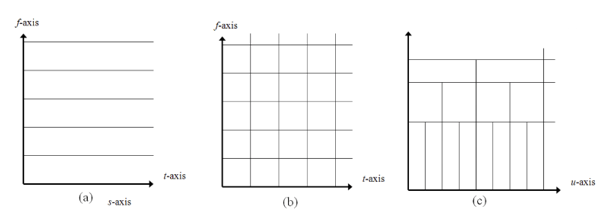
\includegraphics[width=14cm]{thesis/images/tftile}\\
  \caption{Time frequency tiling for (a) Fourier Transform (b) Short-time Fourier Transform (STFT) (c) Wavelet transform}\label{fig_4_2_tftile}
\end{figure}

It can be seen here that for the Fourier transform there is no time information obtained.  In the STFT, as there is no way of telling where in time the frequencies are contained, the STFT makes a blanket range of the resolution of the window and is therefore equally tiled potentially losing information based on this setup.  For the case of the wavelet, because it is a scaled and shifted convolution, it takes care of the this problem providing a good resolution in both time and frequency.  The fundamental representation of the continuous wavelet function is:
\begin{equation}
C(a,b)=\int f(t)\frac{1}{\sqrt{a}}\psi\left(\frac{t-b}{a}\right)dt\label{eqn_c4_wavelet01}
\end{equation}
In this equation, $a$ and $b$ respectively represent the scaling and shifting resolution variables of the wavelet function. This is referred to as a mother wavelet. A few other mother wavelet functions discussed later in this chapter. Generally a mother wavelet is identified as being energy spikes in an infinite signal whose accumulative energy sums to zero.

\section{Discrete and Fast wavelet transform}
Synthesis and analysis equations (\ref{eqn_c4_fourier02} and \ref{eqn_c4_fourier01}) can be formulated as a linear combination of the basis $\phi_k(t)$ such that the basis, $\phi_k(t)=e^{j2\pi kt}$, and it's conjugate or orthonormal basis, $\tilde{\phi}_k(t)=e^{-j2\pi kt}$, equations (\ref{eqn_c4_fourier02} and \ref{eqn_c4_fourier01}) now become

\begin{equation}
x(t)=\sum_{k}a_k\phi_k
\label{eqn_c4_dwt02}
\end{equation}

\begin{equation}
a_k=\int x(t)\tilde{\phi}_k(t)
\label{eqn_c4_dwt01}
\end{equation}

With respect to scaling and shifting variables of continuous wavelet transforms in equation (\ref{eqn_c4_wavelet01}), a similar linear combination transformation can be applied by constructing orthonormal bases parameters, referred to as scaling ($\phi$) and translating ($\psi$) functions. For example, a simple Haar mother wavelet transform associated with a delta function, it is seen that:
\begin{equation}
\phi_{j,k}(t)=2^{j/2}\phi(2^jt-k)
\label{eqn_c4_dwt03}
\end{equation}
\begin{equation}
\psi_{j,k}(t)=2^{j/2}\psi(2^jt-k)
\label{eqn_c4_dwt04}
\end{equation}
where j is associated with the dilation (scaling) parameter and k is associated with the position (shifting) parameter. If the Haar coefficients $h_{(\cdot)}[n]=\{1/\sqrt{2},1/\sqrt{2}\}$ are extracted we have the following dilation and position parameters.
\begin{equation}
\phi(t)=h_\phi[n]\sqrt{2}\phi(2t-n)
\label{eqn_c4_dwt05}
\end{equation}
\begin{equation}
\psi(t)=h_\phi[n]\sqrt{2}\psi(2t-n)
\label{eqn_c4_dwt06}
\end{equation}

For any signal, a discrete wavelet transform in $l^2(\mathbb{Z})^1$ can be approximated by
\begin{equation}
f[n]=\frac{1}{\sqrt{M}}\sum_kW_\phi[j_0,k]\phi_{j_0,k}[n]+\frac{1}{\sqrt{M}}\sum_{j=j_0}^\infty\sum_kW_\psi[j,k]\psi_{j,k}[n]
\label{eqn_c4_dwt07}
\end{equation}
Here $f[n],\phi_{j_0,k}[n]$ and $\psi_{j,k}[n]$ are discrete functions defined in [0,M - 1], having a total of M points.  Because the sets $\{\phi_{j_0,k}[n]\}_{k\in\mathbf{Z}}$ and $\{\psi_{(j,k)\in\mathbf{Z}^2,j\ge j_0}\}$ are orthogonal to each other.  We can simply take the inner product to obtain the wavelet coefficients.
\begin{equation}
W_\phi[j_0,k]=\frac{1}{\sqrt{M}}\sum_nf[n]\phi_{j_0,k}[n]
\label{eqn_c4_dwt08}
\end{equation}
\begin{equation}
W_\psi[j,k]=\frac{1}{\sqrt{M}}\sum_nf[n]\psi_{j,k}[n] \quad j\ge j_0
\label{eqn_c4_dwt09}
\end{equation}
Equation (\ref{eqn_c4_dwt08}) is called approximation coefficient while (\ref{eqn_c4_dwt09}) is called detailed coefficients.

These two components show that the approximation coefficient, $W_\phi[j_0,k]$, models a low pass filter and the detailed coefficient,$W_\psi[j_0,k]$, models a high pass filter. It is possible to determine the approximation and detailed coefficients without the scaling and dilating parameters. The resulting coefficients, called the fast wavelet transform, are a convolution between the wavelet coefficients and a down-sampled version of the next order coefficients.  The fast wavelet transform was first postulated in \citep{mallat1989theory}.
\begin{equation}
W_\phi[j,k]=h_\phi[-n]\ast W_\phi[j+1,n]|_{n=2k, k\ge 0}
\label{eqn_c4_dwt10}
\end{equation}
\begin{equation}
W_\psi[j_0,k]=h_\psi[-n]\ast W_\phi[j+1,n]|_{n=2k, k\ge 0}
\label{eqn_c4_dwt11}
\end{equation}

For analysis of the Haar wavelet and the derivation of equations (\ref{eqn_c4_dwt10} and \ref{eqn_c4_dwt11}) see appendix \ref{app01}.

\section{Mel filter banks}

The Fourier and wavelet transform are general means of extracting information from continuous signals using the frequency domain and in the case of the Wavelet transform using both time and frequency domain.  The objective in machine learning, however, is to extract patterns from the derived information.  In this chapter, in particular, the Mel filter bank and the scatter transform are elaborated on as speech feature extractors.  They process high dimensional information obtained from the Fourier and wavelet transform signal processing techniques and reducing the information obtained as lower dimension features.  All this aimed towards loss-less encoding of speech signals relevant for speech recognition.

The Mel filter banks form the basis of the Mel Frequency Cepstral Coefficients (MFCCs) described by \citep{davis1980comparison}.  MFCCs are state-of-the-art speech feature engineering drivers behind automatic speech recognition acoustic models.  Other common speech features used in speech recognition include, Linear Prediction Coefficients (LPCs) and Linear Prediction Cepstral Coefficients (LPCCs),Perceptual Linear Prediction coefficients (PLP),  \citep{mcloughlin2009applied, dines2010measuring}.  The following paragraphs describe how the Mel filters are derived. 

The Mel scale as described by \cite{stevens1937scale} is a perceptual scale which measures sound frequencies as perceived by human subjects equidistant from a sound source as compared to the actual frequency.  This scale is non-linear as the human ear processes sound non-linearly both in frequency as well as amplitude.

For the case of frequency, the human ear can discriminate lower frequencies more accurately than the higher frequencies.  The Mel scale model this behaviour by utilising frequency bins.  The frequency bin ranges are narrow at low frequencies and become wide in higher frequencies. In the case of the speech signal amplitude, a similar process is observed where the ear discriminates softer sounds better than louder sounds.  Generally, sound will be required to be 8 times as loud for significant perception by the ear.  While the Mel scales handle the frequency non-linearity in the speech signal, the signal amplitude is linearised during feature extraction by taking the log of the power spectrum of the signal, also known as the cepstral values.  Furthermore, using a log scale also allows for a channel normalisation technique that employs cepstral mean subtraction. \citep{becchetti1999behaviour}.

The minimum frequency number of bins used for the Mel scale is 26 bins. In order to determine the frequency ranges we use the following formula to convert between the Mel scale and the regular frequency scale:
\begin{equation}
M(f)=1125\ln(1+f/700)
\label{eqn_c4_mel01}
\end{equation}
\begin{equation}
M^{−1}(m)=700\exp(m/1125)−1
\label{eqn_c4_mel02}
\end{equation}
A simple approximation for the Mel scale is obtained by applying linear scale for the first ten filters and for the first 1kHz of the speech frequency range then applying the following formula for the rest (Becchetti, 1999)\citep{becchetti1999behaviour}:
\begin{equation}
\Delta_m=1.2\times \Delta_{m-1}
\label{eqn_c4_mel03}
\end{equation}
where $m$ is the frequency bin index and  $\Delta_m$ is the frequency range between the start and end frequencies for the $m$-th bin. The resulting filters are overlapping filters shown in figure \ref{fig_4_3_mfilt}.
\begin{figure}
\centering
  % Requires \usepackage{graphicx}
  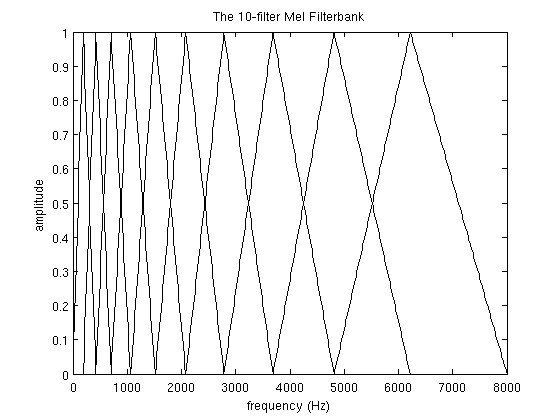
\includegraphics[width=14cm]{thesis/images/m-filters}\\
  \caption{Mel filter plot \citep{lyons_2012}}\label{fig_4_3_mfilt}
\end{figure}
For speech recognition, we compute a statistical value or coefficient for each Mel frequency bin from the inverse discrete fourier transform (IDFT) of the Mel filters.  The coefficients are also concatenated with their delta and delta-delta values.  The delta and delta-delta values are determined from the following equation:
 \begin{equation}
d_t=\frac{\sum_{n=1}^Nn(c_{t+n}−c_{t−n})}{2\sum_{n=1}^Nn^2}
\label{eqn_c4_mel04}
\end{equation}
where $c_x$ is the $x$-th coefficient and $2n$ is the delta range which is usually $2-4$. The delta values are first order derived coefficients obtained from the original Mel filter coefficients while the delta-delta values are second-order derived coefficients obtained from the first-order derived delta coefficients.

There are two reasons for obtaining the IDFT from the filter banks.  The first is that since the bins use overlapping windows, the filter bin outputs tend to be correlated and obtaining the IDFT helps to decorrelate the outputs.  Secondly, decorrelated signals optimise algorithm computation efficiency involving matrix operations such that rather than using full co variance matrix, it is much simpler to compute the matrix operations from the matrix diagonal.  Also note that for cepstral values obtained from taking the log of the power power spectrum, the discrete cosine transform (DCT) is used to obtain the IDFT.  This is as a result of the cepstral values being real and symmetric\citep{gales2008application}.

As an attempt for MFCCs to incorporate dynamic frequency changes of the signal, the deltas and the delta-deltas are obtained from the coefficient computation in equation \ref{eqn_c4_mel04}.  However, it is worthy to note that only the first 13 of the coefficients and the resulting dynamic coefficients are used as speech features as it is observed that higher frequency dynamic coefficients rather degrade ASR performance \citep{gales2008application}.

\section{Deep scattering spectrum}
In this section reference is made to \citep{anden2011multiscale, anden2014deep, zeghidour2016deep}. For a signal $x$ we define the following transform $W_x$ as a convolution with a low-pass filter $\phi$ and higher frequency complex analytic wavelets $\psi_{\lambda_1}$:
\begin{equation}
Wx=(x\star\phi(t),x\star\psi_{\lambda_1}(t))_{t\in\mathbb{R},\lambda_1\in\Lambda_1} \label{eqn_c4_dss01}
\end{equation}

We apply a modulus operator to the wavelet coefficients to remove complex phase and extract envelopes at different resolutions
\begin{equation}
|W|x=\left(x\star\phi(t),|x\star\psi_{\lambda_1}(t)|\right)_{t\in\mathbb{R},\lambda_1\in\Lambda_1} \label{eqn_c4_dss02}
\end{equation}
$S_0x=x\star\phi(t)$ is locally invariant to translation thanks to the time averaging $\phi$.  This time-averaging loses the high frequency information, which is retrieved in the wavelet modulus coefficients $|x\star\psi_{\lambda_1}|$.  However, these wavelet modulus coefficients are not invariant to translation, and as for $S_0$, a local translation invariance is obtained by a time averaging which defines the first layer of scattering coefficients
\begin{equation}
S_1x(t,\psi_{\lambda_1})=|x \star\psi_{\lambda_1}| \star\phi(t)\label{eqn_c4_dss03})
\end{equation}
It is shown in \cite{anden2014deep} that if the wavelets $\psi_{\lambda_1}$ have the same frequency resolution as the standard Mel-filters, then the $S_1x$ coefficients approximate the Mel-filter coefficients.  Unlike the Mel-filter banks however, there is a strategy to recover the lost information, by passing the wavelet modulus coefficients  $|x\star\phi_{\lambda_1}|$ through a bank of higher frequency wavelets $\psi_{\lambda_2}$:
\begin{equation}
|W_2||x\star\phi_{\lambda_1}|=\left(|x\star\psi_{\lambda_1}|\star\phi,||x\star\psi_{\lambda_1}|\star\psi_{\lambda_2}|\right)_{\lambda_2\in\Lambda_2} \label{eqn_c4_dss04})\end{equation}
This second layer of wavelet modulus coefficients is still not invariant to translation, hence we average these coefficients with a low-pass filter $\phi$ to derive a second layer of of scattering coefficients.
 \begin{equation}
|W_2||x\star\phi_{\lambda_1}|=\left(|x\star\psi_{\lambda_1}|\star\phi,||x\star\psi_{\lambda_1}|\star\psi_{\lambda_2}|\right)_{\lambda_2\in\Lambda_2}\label{eqn_c4_dss04})\end{equation}

Repeating these successive steps of computing invariant features and retrieving lost information leads to the scattering spectrum, as seen in Fig. 1, however speech signals are almost entirely characterized by the first two layers of the spectrum, that is why a two layers spectrum is typically used for speech representation. It is shown in [6] that this representation is invariant to translations and stable to deformations, while keeping more information than the Mel-filter banks coefficients
\begin{figure}
\centering
  % Requires \usepackage{graphicx}
  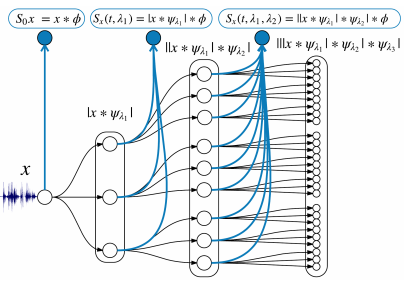
\includegraphics[width=14cm]{thesis/images/scatter.png}\\
  \caption{Scattering network - 2 layers deep} \cite{zeghidour2016deep}\label{fig_4_3_scatter}
\end{figure}
